\chapterimage{onions.jpg}


\chapter{A Stack of Layers}\label{sec:stack_layers}

Modern computer communication is achieved using a
\concept{stack} of network \conceptRef{layer}{layers}.
Each stack focuses on some problems and is responsible for 
providing certain features, \eg, 
\conceptRef{address}{addressing} and correct \concept{sequencing} (introduced in the previous chapters).

Each \concept{layer} defines a \inlineCode{send}/\inlineCode{receive} function \textit{pair},
which is responsible for some of these features.
% 
Each layer uses the \inlineCode{send} and \inlineCode{receive} of the layer below,
\ie, the features of one layer rely on the features of all layers below it.

To coordinate layers and enable \concept{virtual} communication between them, 
each layer defines a different \concept{packet format}, which \conceptRef{encapsulation}{encapsulates} 
a packet of the layer above it.


\section{Sending data}

To implement these 
capabilities, each layer transmits not only the \inlineCode{data} provided by the layer above, 
but also a header with all the meta-information required for that capability. Thus, each layer needs to define
the \concept{packet format}, adding some \concept{overhead} (typically a \concept{header}) to the \concept{payload}, \eg:

\begin{center}
    \begin{bytefield}{36}
     \bitbox{12}{Header} & \bitbox{24}{Payload}
    \end{bytefield}
\end{center}



When a user program wants to send some data, it uses the \inlineCode{send} method of the \textit{top} layer of the stack,
which eventually results in some data being transmitted by the physical layer, \eg, through a cable or antenna.
The following figure depicts the structure of a 4-layer \concept{stack}:

\begin{center}
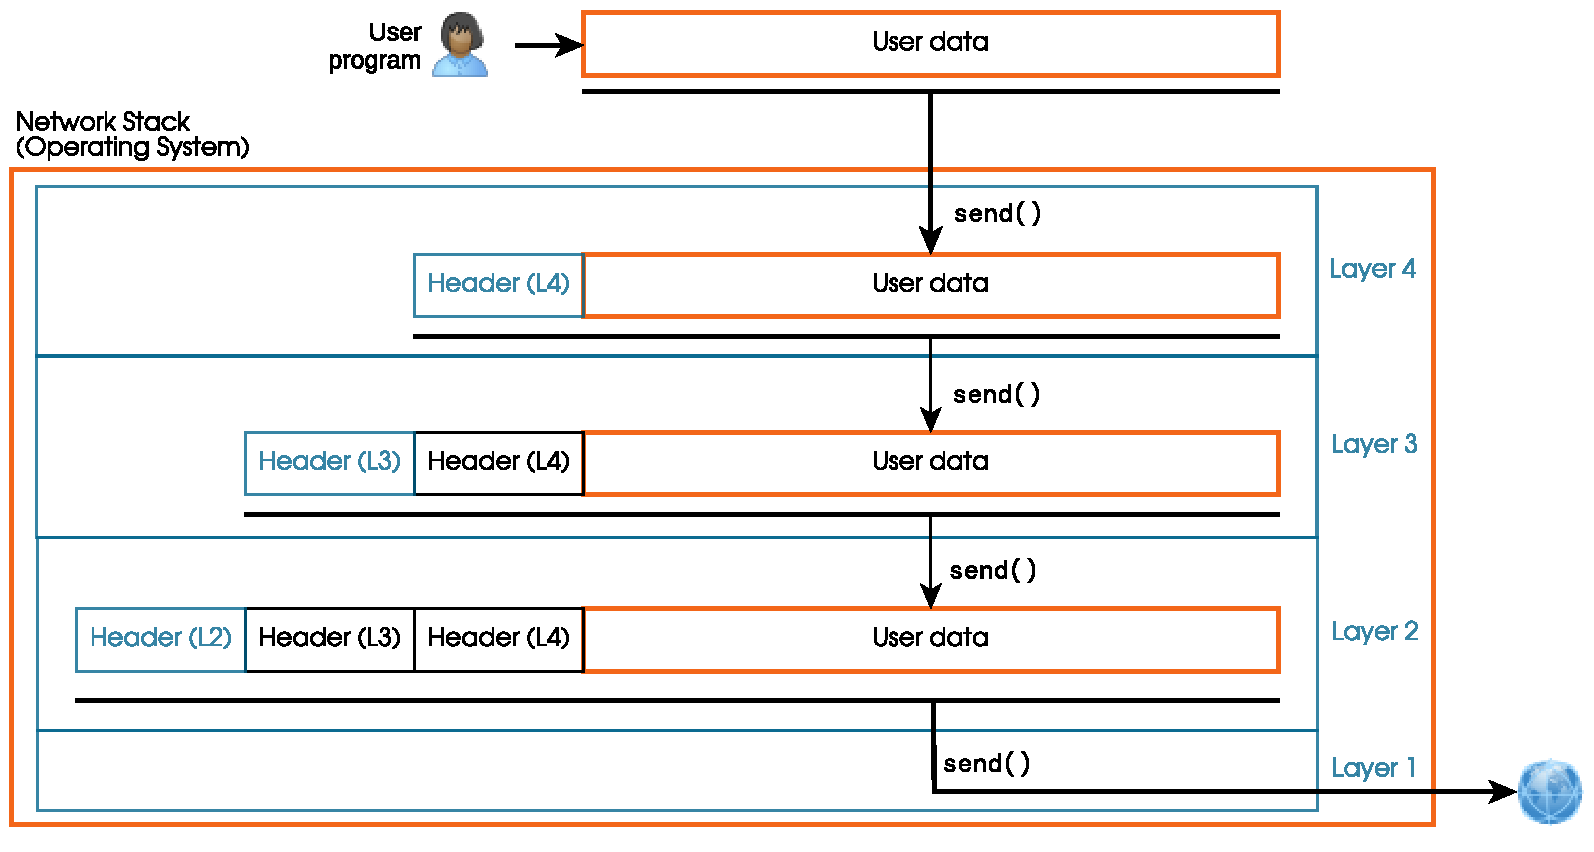
\includegraphics[width=\linewidth]{encapsulation_send.pdf}
\end{center}


The packets produced by each layer are generically referred to as \concept{PDU}s (Protocol Data Unit).
The PDUs of each layer have specific names such as \concept{frame}, \concept{datagram} or \concept{segment}.
These names must be used with precision in technical contexts.

Each layer includes the \concept{PDU} of the layer above inside its PDU's \concept{packet format} definition.
This process is referred to as \concept{encapsulation}.

\begin{exercise}

The user program wants to send $420$~bytes of data using the \concept{stack} of the previous figure.
Assume a header size for layers 2, 3 and 4 of $14$~bytes, $20$~bytes and $20$~bytes, respectively.
\begin{itemize}
    \item What is the \concept{payload} size and the \concept{overhead} size for each \concept{layer}'s \concept{PDU}?
    \item What is the \concept{payload} size and the \concept{overhead} size of the whole \concept{stack}?
\end{itemize}
\end{exercise}

\section{Receiving data}

When a \concept{packet} reaches the network \concept{stack} of the recipient, it is processed in reverse order,
\ie, layers are traversed from bottom to top. Each layer inspects \textit{only} the \concept{header} corresponding to that layer.
If everything is correct, the layer removes the header and passes the remainder of the packet to the layer above.
In turn, the layer on top passes the remaining data (the \concept{payload}) to the recipient.
Continuing the example of the 4-layer stack:

\begin{center}
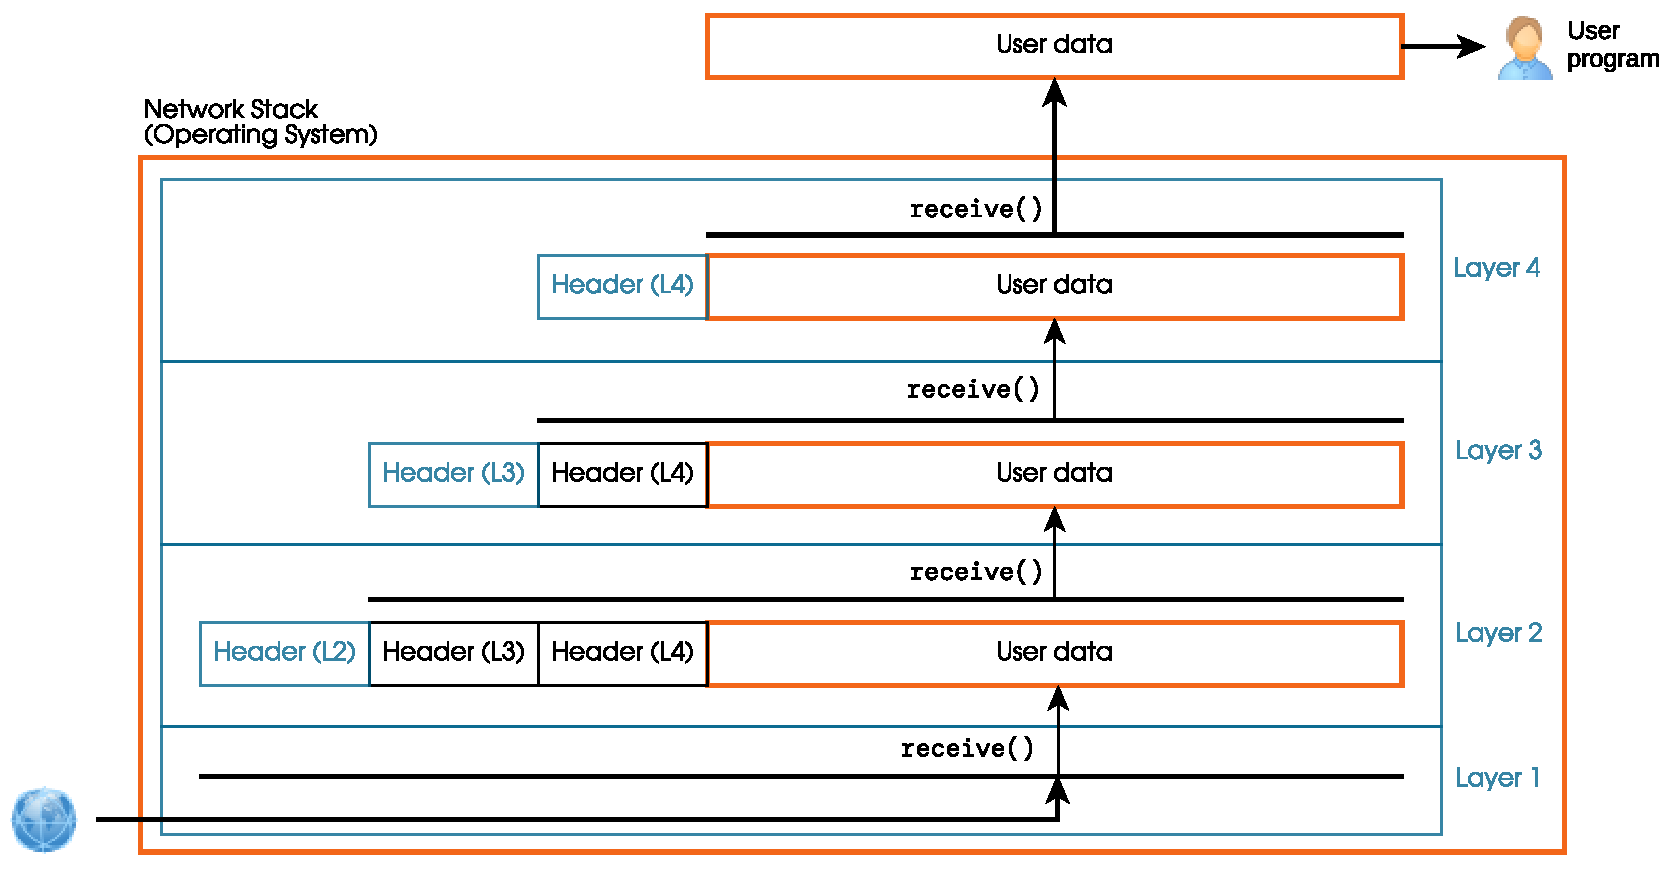
\includegraphics[width=\linewidth]{encapsulation_receive.pdf}
\end{center}


In a \conceptRef{stack}{network stack}, only the bottom layer interacts directly with the exterior,
\eg, only the physical network card of a computer is connected to a wire that carries data to other computers.
% 
At the same time, data sent by the bottom layer includes the \conceptRef{PDU}{PDUs} of all layers
by means of \concept{encapsulation}.
% 
Thanks to this, there exists a \concept{virtual} communication between each layer in one end and its counterpart in the other 
end of communication. The following figure represents the real (solid line) and virtual (dashed line) communication 
in our example:

\begin{center}
    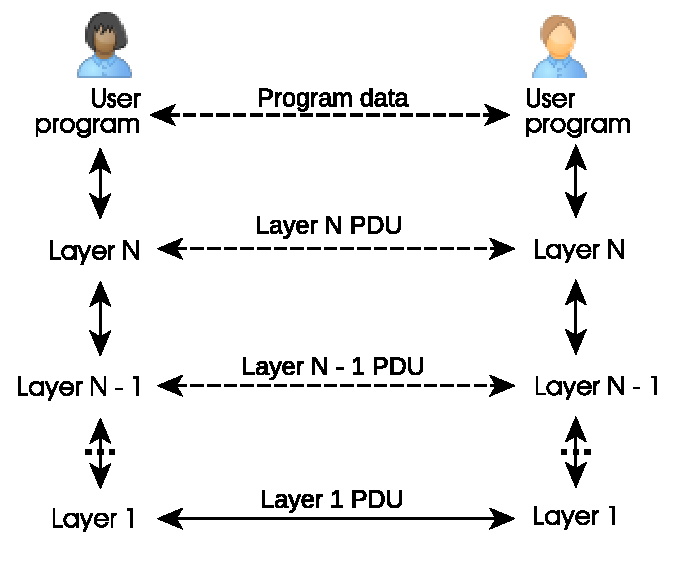
\includegraphics[width=0.5\linewidth]{horizontal_layer_communication.pdf}
\end{center}


\begin{exercise}
Another network \concept{stack} example has 3 layers: L1, L2 and L3 from bottom to top.

The \concept{PDU} of layer L2 is as follows:

\begin{center}
\begin{bytefield}{32}
\bitheader{0,7,8,15,16,23,24,31}\\
\bitbox{16}{Destination address} & \bitbox{16}{Payload length (bytes)} \\
\wordbox{2}{{Payload (variable length)\\$\vdots$}}
\end{bytefield}
\end{center}

The \concept{PDU} of layer L3 is as follows:

\begin{center}
\begin{bytefield}{32}
\bitheader{0,7,8,15,16,23,24,31}\\
\bitbox{16}{Fragment offset} & \bitbox{16}{Payload length (bytes)} \\
\wordbox{2}{{Payload (variable length)\\$\vdots$}}
\end{bytefield}
\end{center}

Layer L1 receives a \concept{packet} of data and its \inlineCode{receive} function returns the following data
(assume \concept{unsigned} integers and \concept{big endian} order when needed:
\begin{center}
\otherBase{01 23 00 0a 01 00 00 06 00 aa 00 bb 43 20}
\end{center}
\begin{itemize}
\item What data \concept{payload} was sent to the recipient program in this \concept{packet}?\\[-0.25cm]

\item If this is the last \concept{packet} of the communication, how much (\concept{payload}) data was sent
  to the recipient user program?\\[-0.25cm]
  
\item At most, how many different computers can connect using this \concept{stack}?\\[-0.25cm]

\item We send a file as the payload of this stack. What's its maximum possible size?
\end{itemize}
\label{ex:how_it_is_done:three_layer_network}
\end{exercise}

\begin{center}
\showCode{snippets/encapsulation.py}
\end{center}

\begin{exercise}
The previous code takes some data and writes the bytes that would be sent to Layer 1 
(the \concept{physical layer}) of the \concept{network stack} of Exercise~\ref{ex:how_it_is_done:three_layer_network}.
Implement the receiving end of the stack as follows: 

\begin{itemize}
\item Implement a \inlineCode{layer2_decapsulate(data: bytes) -> (int, bytes)} function that takes a Layer 2 PDU
  and returns the tuple \inlineCode{(address, payload)}, where \inlineCode{address} is the destination address and 
  \inlineCode{payload} is the encapsulated Layer 3 PDU.\\[-0.25cm]
  
\item Implement a \inlineCode{layer3_decapsulate(data: bytes) -> (int, bytes)} function that takes a Layer 3 PDU
  and returns the tuple \inlineCode{(offset, payload)}, where \inlineCode{offset} is the payload offset, and 
  \inlineCode{payload} is the chunk of data sent by the other end of communication.\\[-0.25cm]
  
\item Implement a \inlineCode{stack_receive(data: bytes)} function that decodes a Layer 1 PDU (using the two previous functions)
  and prints a message line similar to 
  \begin{center}
  \inlineCode{"Received a chunk of data. Length: 12 bytes, Address: 0xabcd, Offset: 0."}
  \end{center}\ \\[-0.75cm]
  
\item Complete the \inlineCode{stack_send} function so that the input data are split in chunks of at most 100 bytes, 
      a valid Layer 1 PDU is produced for each of those chunks,
      and those Layer 1 PDUs are passed to \inlineCode{stack_receive}.\\[-0.25cm]
      
\item Would your implementation work if the Layer 1 PDUs were randomly ordered before passing them to the receiving stack?
\end{itemize}
% 
\label{ex:how_it_is_done:implementation_three_layer_network}
\end{exercise}

\begin{remark}
Python's \inlineCode{struct} library is useful, but not mandatory, to format \concept{packet} bytes.
\end{remark}
